\documentclass[aspectratio=169,10pt]{beamer}

\usetheme{Madrid}
\usecolortheme{default}
\setbeamertemplate{navigation symbols}{}
\setbeamertemplate{footline}[frame number]

\usepackage{amsmath,amssymb,amsthm,booktabs,mathtools}
\usepackage{stmaryrd}
\usepackage{graphicx}
\usepackage{hyperref}
\usepackage{tikz}
\usetikzlibrary{arrows.meta,positioning,decorations.pathreplacing}
\usepackage{subcaption}

% Semantic colors
\definecolor{positive}{HTML}{0173B2}
\definecolor{negative}{HTML}{DE8F05}
\definecolor{emphasis}{HTML}{029E73}
\definecolor{neutral}{gray}{0.55}
\definecolor{cbPurple}{HTML}{CC78BC}
\newcommand{\pos}[1]{\textcolor{positive}{#1}}
\newcommand{\con}[1]{\textcolor{negative}{#1}}
\newcommand{\HL}[1]{\textcolor{emphasis}{#1}}

\author{Pattern Recognition — Final Slide}
\institute{University of Science, VNU HCMC}
\title{Section 5.3 — Analysis}
\subtitle{Adaptive Normalized Representation Learning for Generalizable Face Anti-Spoofing}
\date{}

\begin{document}

% ─────────────────────────────────────────────────────────
% Slide 1 — Title
% ─────────────────────────────────────────────────────────
\begin{frame}
  \titlepage
\end{frame}

% ─────────────────────────────────────────────────────────
% Slide 2 — Outline
% ─────────────────────────────────────────────────────────
\begin{frame}{Outline}
  \begin{columns}[T]
    \column{0.48\textwidth}
      \vspace{6pt}
      \begin{block}{5.3.1 Feature Map Analysis}
        \begin{itemize}
          \item CNN feature map formulation
          \item High vs. low weight channels
          \item Adaptive feature combination
        \end{itemize}
      \end{block}
    \column{0.48\textwidth}
      \vspace{6pt}
      \begin{block}{5.3.2 Balance Factor Analysis}
        \begin{itemize}
          \item Layer-wise $\alpha$ behavior
          \item Sample-adaptive normalization
          \item Domain discrepancy effect
        \end{itemize}
      \end{block}
  \end{columns}
  \vspace{10pt}
  \begin{center}
    \pos{$\blacktriangleright$} Both analyses explain \HL{why} AFNM generalizes better than fixed-normalization baselines.
  \end{center}
\end{frame}

% ─────────────────────────────────────────────────────────
% Slide 3 — Feature Map Analysis: CNN Basics
% ─────────────────────────────────────────────────────────
\begin{frame}{Feature Map Analysis: CNN Feature Representation}
  \textbf{Feature maps} = intermediate activations capturing edges, textures, semantic structures.

  \vspace{8pt}
  A convolutional layer applies learnable filters to produce output feature maps:
  \[
    F_k = \sigma(W_k \ast X + b_k)
  \]
  \begin{description}
    \item[$W_k, b_k$] weights and bias of the $k$-th filter
    \item[$\ast$] convolution operation
    \item[$\sigma(\cdot)$] non-linear activation
    \item[$X \in \mathbb{R}^{C \times H \times W}$] input feature tensor
  \end{description}

  \vspace{6pt}
  In AFNM, each channel is normalized via a \HL{balance-weighted combination} of BatchNorm and InstanceNorm:
  \[
    \hat{x}_c = \underbrace{(1-\alpha_c)}_{\text{IN weight}} \cdot \text{IN}(x_c)
               + \underbrace{\alpha_c}_{\text{BN weight}} \cdot \text{BN}(x_c)
  \]
  The scalar $\alpha_c$ is \pos{learned per sample and channel}.
\end{frame}

% ─────────────────────────────────────────────────────────
% Slide 4 — Feature Map Analysis: Visual Evidence
% ─────────────────────────────────────────────────────────
\begin{frame}{Feature Map Analysis: High vs. Low Weight Channels}
  \begin{columns}[T]
    \column{0.55\textwidth}
      \begin{figure}
        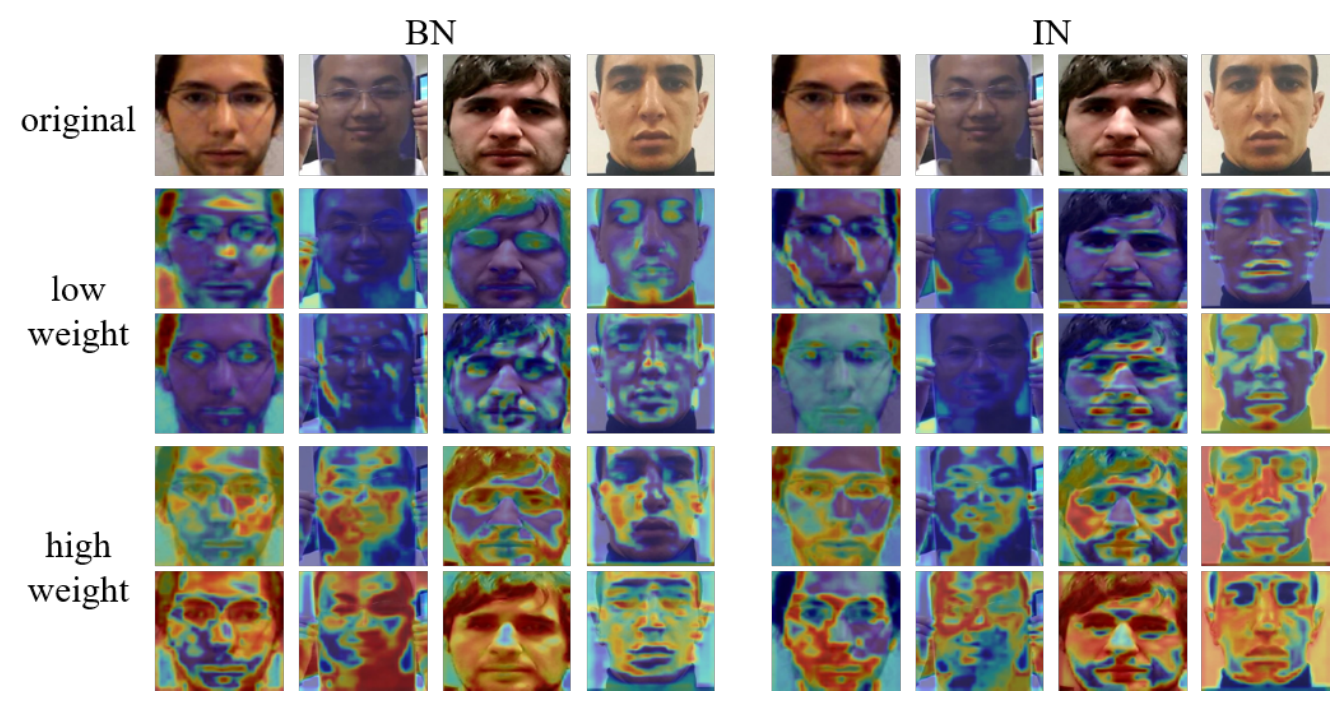
\includegraphics[width=\textwidth]{img/fig15-feature-maps-low-high-weight.png}
        \caption{Feature maps of low/high-weight channels (IN and BN)}
      \end{figure}
    \column{0.42\textwidth}
      \small
      \vspace{6pt}
      \textbf{Key observations:}

      \pos{$\bullet$ High-weight channels} (large $\alpha$)
      \begin{itemize}
        \item Focus on \HL{facial regions}
        \item Capture intrinsic spoofing cues
        \item Transferable across domains
      \end{itemize}

      \con{$\bullet$ Low-weight channels} (small $\alpha$)
      \begin{itemize}
        \item Capture background / artifacts
        \item Domain-specific noise
      \end{itemize}

      \vspace{6pt}
      AFNM \HL{suppresses domain noise}, preserves discriminative info $\Rightarrow$ better generalization.
  \end{columns}
\end{frame}

% ─────────────────────────────────────────────────────────
% Slide 5 — Feature Map Analysis: Fusion Visualization
% ─────────────────────────────────────────────────────────
\begin{frame}{Feature Map Analysis: Weighted Fusion}
  \begin{columns}[T]
    \column{0.55\textwidth}
      \begin{figure}
        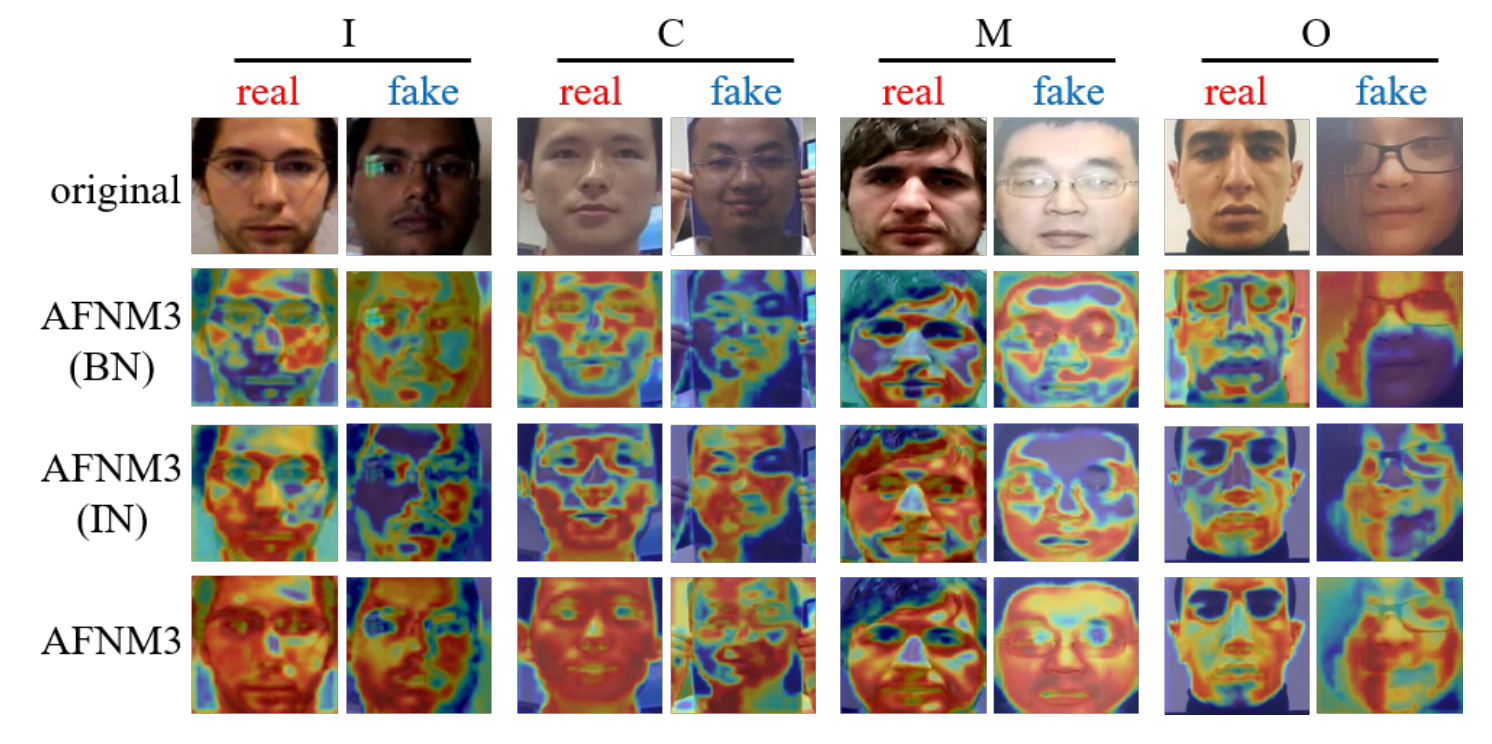
\includegraphics[width=\textwidth]{img/fig16-weighted-feature-maps-fusion.png}
        \caption{Weighted BN, IN channels and their fusion (AFNM3, task I\&C\&M $\to$ O)}
      \end{figure}
    \column{0.42\textwidth}
      \small
      \vspace{6pt}
      BN and IN channels are combined per channel with learned weights.

      \vspace{6pt}
      \begin{block}{Why fusion works}
        \begin{itemize}
          \item BN captures \HL{class-discriminative} features
          \item IN removes \HL{domain-specific} variations
          \item Adaptive weighting selects the right balance per sample
        \end{itemize}
      \end{block}

      \vspace{6pt}
      The fused representation is \HL{less sensitive to domain shift} while retaining spoofing-sensitive patterns.
  \end{columns}
\end{frame}

% ─────────────────────────────────────────────────────────
% Slide 6 — Balance Factor: Layer-wise Behavior
% ─────────────────────────────────────────────────────────
\begin{frame}{Balance Factor $\alpha$: Layer-wise Behavior}
  \begin{columns}[T]
    \column{0.58\textwidth}
      \begin{figure}
        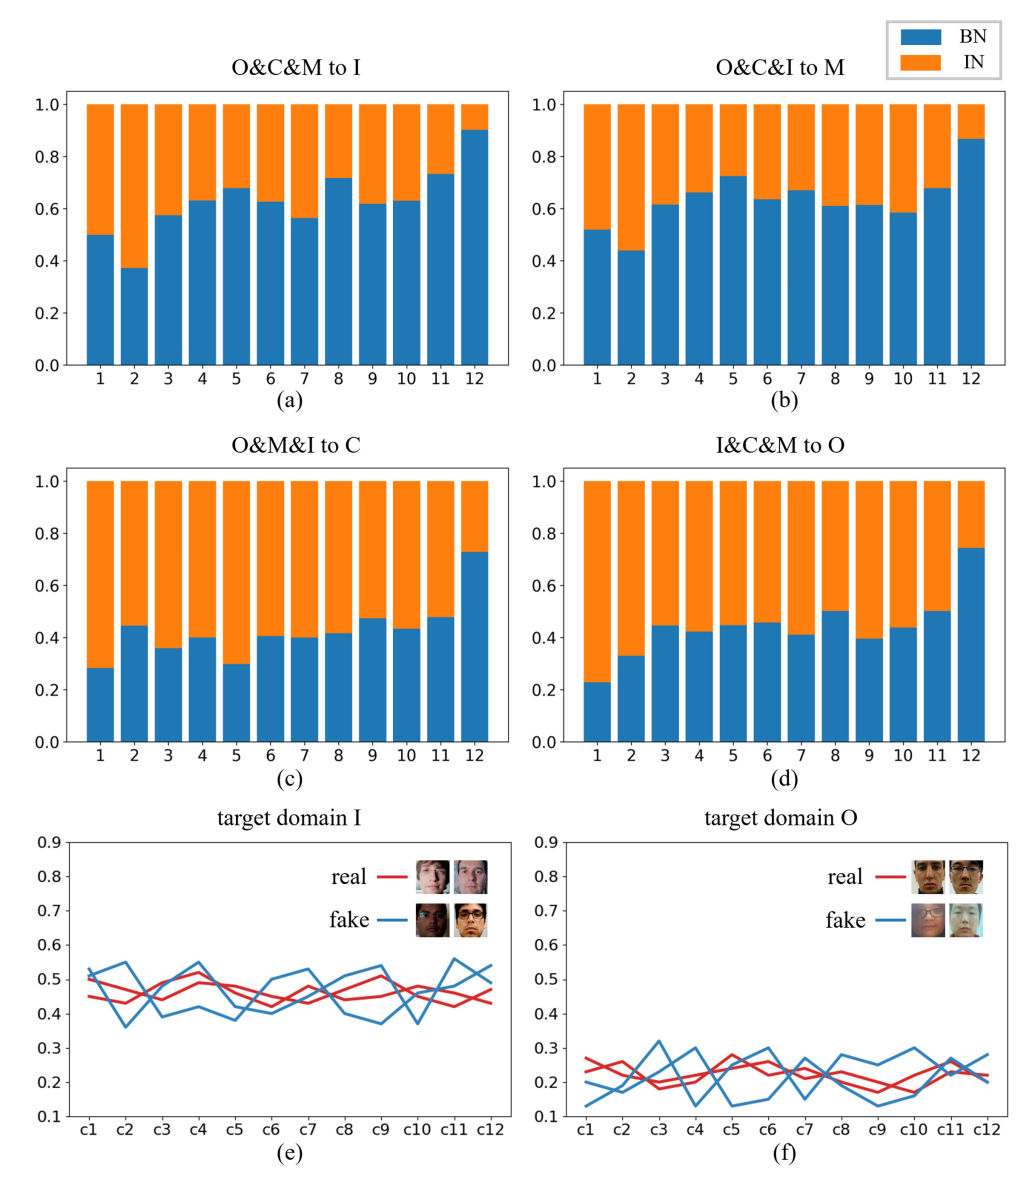
\includegraphics[width=\textwidth]{img/fig17-balance-factor-alpha.png}
        \caption{Mean balance factor $\alpha$ per layer across 4 testing tasks}
      \end{figure}
    \column{0.39\textwidth}
      \small
      \vspace{6pt}
      $\alpha$ controls BN vs. IN contribution:

      \begin{block}{Shallow layers ($L_1, L_2$)}
        $\alpha \approx 0$ \pos{small}

        \hspace{4pt}IN dominates $\Rightarrow$ removes domain-specific variations
      \end{block}

      \begin{block}{Deep layers ($L_3, L_4$)}
        $\alpha \to 1$ \pos{large}

        \hspace{4pt}BN dominates $\Rightarrow$ extracts high-level discriminative features
      \end{block}

      \vspace{4pt}
      \HL{Task with larger domain discrepancy} $\Rightarrow$ more IN reliance ($\alpha$ lower overall).
  \end{columns}
\end{frame}

% ─────────────────────────────────────────────────────────
% Slide 7 — Balance Factor: Sample Adaptation + t-SNE
% ─────────────────────────────────────────────────────────
\begin{frame}{Balance Factor $\alpha$: Sample Adaptation and Feature Geometry}
  \begin{columns}[T]
    \column{0.58\textwidth}
      \begin{figure}
        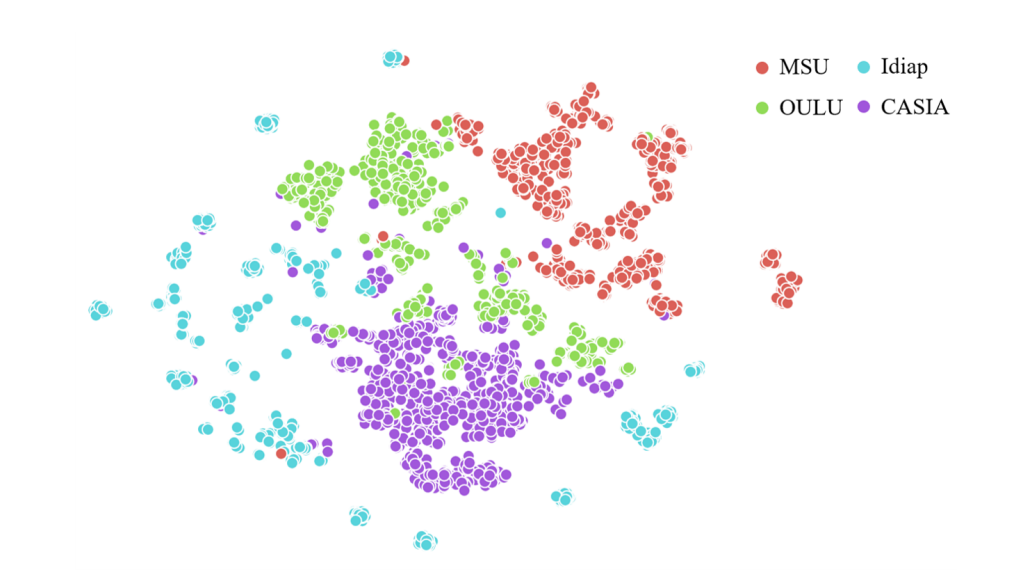
\includegraphics[width=\textwidth]{img/fig18-tsne-visualization.png}
        \caption{t-SNE visualization of features from ResNet (ImageNet pretrained)}
      \end{figure}
    \column{0.39\textwidth}
      \small
      \vspace{6pt}
      \textbf{Sample-adaptive normalization:}

      \begin{itemize}
        \item $\alpha$ varies \HL{significantly across samples}
        \item Model adjusts strategy per input
        \item Handles diverse attack types and domain shifts
      \end{itemize}

      \vspace{6pt}
      \textbf{t-SNE insight:}

      \begin{itemize}
        \item Real vs. fake samples are \HL{more separable} with AFNM
        \item Feature clusters are \pos{more compact} across domains
      \end{itemize}

      \vspace{6pt}
      Confirms adaptive normalization improves \HL{cross-domain discriminability}.
  \end{columns}
\end{frame}

% ─────────────────────────────────────────────────────────
% Slide 8 — Summary
% ─────────────────────────────────────────────────────────
\begin{frame}{Summary: Key Takeaways from Section 5.3}
  \begin{enumerate}
    \item \textbf{Feature maps} from CNNs encode hierarchical patterns; AFNM adaptively weights channels to suppress domain-specific noise while preserving spoofing cues.

    \item \textbf{High-weight channels} (BN+IN) focus on facial regions; \textbf{low-weight channels} capture background / artifacts — AFNM suppresses the latter.

    \item \textbf{Balance factor $\alpha$} is layer-dependent:
          \pos{shallow $\Rightarrow$ IN} (remove domain variation),
          \pos{deep $\Rightarrow$ BN} (extract discriminative features).

    \item $\alpha$ is \HL{sample-adaptive} — the model tailors normalization per input, which is crucial for handling diverse attack types and domain shifts.

    \item t-SNE confirms AFNM features are \HL{more separable and compact} across domains than fixed-normalization baselines.
  \end{enumerate}

  \vspace{8pt}
  \begin{center}
    \fbox{Adaptive normalization $\Rightarrow$ robust domain generalization for face anti-spoofing.}
  \end{center}
\end{frame}

\end{document}
